%% LaTeX2e class for student theses
%% sections/content.tex
%%
%% Karlsruhe University of Applied Sciences
%% Faculty of  Computer Science and Business Information Systems
%% Distributed Systems (vsys)
%%
%% Prof. Dr. Christian Zirpins
%% christian.zirpins@hs-karlsruhe.de
%%
%%
%% Version 0.2, 2017-11-15
%%
%% --------------------------------------------------------
%% | Derived from sdqthesis by Erik Burger burger@kit.edu |
%% --------------------------------------------------------
\chapter{Entwurf einer Lösung für Server-zu-Server Interaktion mit ActivityPub}
	Zu Beginn dieses Kapitels wird auf die Entwurfsentscheidung eingegangen und folgende Frage beantwortet:
	\begin{itemize}
		\item Warum wurde die im folgenden beschriebene Architektur gewählt?
	\end{itemize}
	Darauffolgend wird konkret auf die technische Architektur eingegangen und mit Diagrammen veranschaulicht wie diese aussieht.
\section{Entwurfsentscheidung}
	Aus Gründen der Einfachheit wurde sich in dieser Arbeit für eine drei Schichten Architektur, bestehend aus Controller-Schicht, Serviceschicht und Datenschicht, entschieden. Hierbei wird die letzte Schicht implementiert und ist somit die Schnittstelle für Entwickler zum integrieren des Frameworks in eine bestehende Applikation. Es wurde sich für die Datenschicht (IDataSource) entschieden um eine breite Fläche an Datenbanken und \gls{api}'s ansprechen zu können; Abhängig davon was bereits besteht.\\
	
	Um außerdem Entwicklern zu ermöglichen auch ohne bestehenden Express Web Server, in den das Framework integriert wird, mit dem implementieren zu beginnen kann der Service ohne Parameter initialisiert werden und startet damit einen separaten Web Server.\\
	
	Ein besseres Codeverständnis wurde erlangt durch die Erstellung einer Fassaden Klasse, welche Weiterleitungen zum Interface enthält. Dabei handelt es sich um Funktionalität welche mit Sammlungen zu tun hat. Die Klasse heißt dementsprechend \glqq Collections\grqq.\\
	
	Außerdem wurde sich für das Erstellen von Nutzern für jeden Aktor des Fediverse, welche mit dieser Instanz kommuniziert, entschieden, da dadurch die automatische Erstellung von Relationen erhalten bleibt. Somit entfallen größere Änderungen am verwendeten Datenschema.
	\pagebreak
\section{Technische Architektur}
	Die technische Architektur ist in drei Schichten aufgeteilt. Der \textit{ Controller}~hat die Aufgabe HTTP Anfragen entgegen zu nehmen. In der \textit{Service} Schicht bekommen alle Methoden eine Aktivität als Parameter übergeben. Zudem nutzen alle Service Methoden die IDataSource Implementierung. Diese stellt die \textit{Datenschicht} dar.\\
	
	Der ActivityPub Service wird als Express Middleware, sowie als allein stehender Web Server bereitgestellt. Bei der letzteren Variante wird anstatt die Middleware in ein bestehenden Express Server zu integrieren, ein eigener  Server gestartet.\\
	\begin{figure}[H]
		\centering
		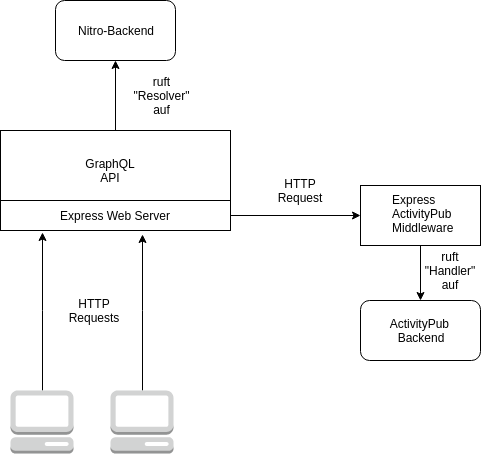
\includegraphics[scale=0.6]{figures/technische-architektur-activitypub.png}
		\label{fig:tech-arch}
		\caption{Technische Architektur ActivityPub}
	\end{figure}
	In der oben gezeigten Abbildung wurde der ActivityPub Service in einen bestehenden Express Server einer GraphQL API integriert.\\
	
	Benutzer der \gls{api} kommunizieren mit dem Web Server über das HTTP Protokoll. Der Web Server leitet die Anfragen dann an den entsprechenden Router weiter, welcher wiederum den Anfrage Inhalt transformiert und \glqq Handler\grqq~Funktionen der Service Schicht, mit entsprechenden Parametern, aufruft.
	\begin{figure}[h]
		\begin{minipage}{\textwidth}
			\centering
			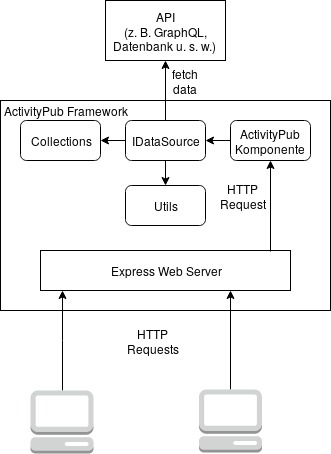
\includegraphics[scale=0.6]{figures/technical-architecture-standalone.png}
			\label{technische-architektur-standalone}
			\caption{Technische Architektur als allein stehender Server}
		\end{minipage}
	\end{figure}
	Die obige Abbildung zeigt eine detailliertere Variante des ActivityPub Service Diagramms aus Abb. 4.1.\\
	
	Der Router stellt hier die Controller Schicht dar bei der die HTTP Anfragen der Nutzer eingehen und die ActivityPub Komponente ist der eigentliche Service und stellt zudem die gleich benannte Schicht dar.\\
	
	Bei der Architektur wird weitestgehend darauf Wert gelegt, dass alle ActivityPub konformen Inhalte dynamisch generiert werden können. Damit wird versucht für bestehende Projekte die diesen Prototypen integrieren wollen einen einfachen Einstieg zu bieten um andere Datenbanken o.ä. anbinden zu können.\\